\subsection{Clase \textit{Infraestructure} y redes de grafos}
    \label{sec:grafos}

    La clase \textit{Infraestructure} define todos los elementos ferroviarios con características físicas, materiales y estáticas. Las clases que contiene son:

    \begin{itemize}
        \item \textit{Topology}: define la topología de la red mediante las clases \textit{netElements} y \textit{netRelationships}. Incluye también la clase \textit{Network} para cumplir con el estándar de RailTopoModel.
        \item \textit{Geometry}: define el sistema geométrico utilizado entre las clases \textit{HorizontalCurve} (en base al largo y el ángulo formado), \textit{GradientCurves} (en base al largo y al gradiente de la curva) y \textit{GeometryPoints} (en base a una combinación de las dos clases anteriores).
        \item \textit{FunctionalInfrastructure}: define todos los elementos ferroviarios que el RNA analizará.
        \item \textit{PhysicalFacilities}: actualmente el estándar lo define vacío, sin ninguna clase interna salvo la clase \textit{Any} que puede ser utilizada como comodín.
        \item \textit{InfrastructureVisualizations}: define las coordenadas y estructura del elemento ferroviario en base a sus clases \textit{tRef} (para indicar a que elemento afecta), \textit{SpotProjection} (coordenada del elemento), \textit{LinearProjection} (en caso de ser un elemento lineal) y \textit{AreaProjection} (en caso de ser un elemento bidimensional).
        \item \textit{InfrastructureStates}: define la validez de los datos referidos a cada elemento ferroviario.
    \end{itemize}

    Para realizar el análisis de la red, el RNA debe centrarse en tres de estas clases: \textit{Topology} (para conocer cómo es la red), \textit{FunctionalInfrastructure} (para conocer qué elementos tiene la red) y \textit{InfrastructureVisualizations} (para conocer dónde está cada elemento ferroviario).

    Empezando por la clase \textit{Topology}, existen dos clases esenciales para este análisis: la clase \textit{netElements} y la clase netRelationships. Ambas son clases vectores, constituidas por clases mas pequeñas: \textit{netElement} y \textit{netRelationship}. Un ejemplo de la clase \textit{netElement} se puede ver en el Código \ref{lst:netElement}.
    
    \begin{lstlisting}[language = XML, caption = Clase \textit{netElement} , label = {lst:netElement}]
<netElement id="ne3">
    <associatedPositioningSystem id="ne3_aps01">
        <intrinsicCoordinate intrinsicCoord="0" id="ne3_aps01_ic01">
            <geometricCoordinate x="9384.050" y="0.000" positioningSystemRef="gps01"/>
        </intrinsicCoordinate>
        <intrinsicCoordinate intrinsicCoord="1" id="ne3_aps01_ic02">
            <geometricCoordinate x="7584.770" y="0.000" positioningSystemRef="gps01"/>
        </intrinsicCoordinate>
    </associatedPositioningSystem>
    <relation ref="nr_ne3ne46_swi77"/>
    <relation ref="nr_ne3ne53_swi77"/>
</netElement>
    \end{lstlisting}
    
    Los elementos mas importantes a destacar en el Código \ref{lst:netElement} son el id, el \textit{geometricCoordinate} y el \textit{relation}. De estos parametros podemos saber que el \textit{netElement} es referido como "ne3", comienza en la coordenada (9384.050 ; 0.000) y termina en la coordenada (7584.770 ; 0.000). Además, ne3 se encuentra relacionado a los \textit{netElement} ne46 y ne53 mediante un elemento referido como swi77, que más adelante veremos que se trata de un cambio de vías.

    Los \textit{netElement} son los nodos de la red de grafos, pero estos no son puntuales, sino que son bidimensionales. Debido a que la componente x de la coordenada de inicio de ne3 es mayor que la componente x de la coordenada final de ne3, podemos deducir que ne3 se encuentra definido de derecha a izquierda. Conocer la orientación del \textit{netElement} será importante a la hora de definir la circulación, información necesaria para generar las rutas.

    La clase \textit{netRelation} son las aristas de la red de grafos que relacionan dos \textit{netElements} entre sí. En el Código \ref{lst:netRelation} se muestra un ejemplo de los \textit{netRelation} que vinculan a los \textit{netElement} ne3, ne46 y ne53.    
    
    \begin{lstlisting}[language = XML, caption = Clase \textit{netRelation} , label = {lst:netRelation}]
<netRelation navigability="Both" positionOnA="1" positionOnB="1" id="nr_ne3ne46_swi77">
    <elementA ref="ne3"/>
    <elementB ref="ne46"/>
</netRelation>
<netRelation navigability="Both" positionOnA="1" positionOnB="1" id="nr_ne3ne53_swi77">
    <elementA ref="ne3"/>
    <elementB ref="ne53"/>
</netRelation>
<netRelation navigability="None" positionOnA="1" positionOnB="1" id="nr_ne46ne53_swi77">
    <elementA ref="ne46"/>
    <elementB ref="ne53"/>
</netRelation>
    \end{lstlisting}
    
    La primer \textit{netRelation} es entre el \textit{netElement} ne3 y el ne46, la segunda \textit{netRelation} es entre el netElement ne3 y el ne53. Esto es consistente con los parámetros de relation que tenía el netElement ne3 en el Código \ref{lst:netElement}. Sin embargo, en el tercer \textit{netRelation} vemos que existe una relación entre los \textit{netElement} ne46 y ne53 pero, en este caso, el parámetro \textit{navigability} es "None", a diferencia de los primeros dos que era "both". La navegabilidad es el parámetro que hace que una red de grafos tenga sentido como red ferroviaria: que exista una conexión no implica que sea físicamente utilizable por un tren, tal como se explicó en la Sección \ref{sec:RTM}.
    
    % Explicar analisis de red de grafos
    La secuencia de análisis de la red de grafos se describe en el Algoritmo \ref{alg:graph_network}. Tanto el Algoritmo \ref{alg:graph_network} como todos los algoritmos pertenecientes al RNA y el ACG fueron diseñados e implementados durante el transcurso del presente doctorado. Estos algoritmos no son parte de ningún estándar ni trabajo previo ajeno a este desarrollo, por lo que son una pieza fundamental y original de esta tesis.    
    
    \begin{algorithm}[H]\captionsetup{labelfont={sc,bf}, labelsep=newline}
    	\caption{Análisis de la red de grafos}
    	\label{alg:graph_network}
    	\begin{algorithmic}
    		\STATE \{nodes\} $\gets$ get\_nodes(netElements)
    		\STATE  order\_nodes(\{nodes\})
    		\STATE \{netPaths\} $\gets$ get\_relations(\{nodes\},netRelations)
    		\STATE \{neighbours\} $\gets$ get\_neighbours(\{netPaths\})
    		\STATE \{switches\} $\gets$ get\_switches(\{nodes\},\{neighbours\})
    		\STATE \{limits\} $\gets$ get\_limits(\{nodes\})
    		\STATE analyze\_connectedness(\{netPaths\})
    	\end{algorithmic}
    \end{algorithm}
    
    El primer paso es procesar la clase \textit{netElements} para obtener un diccionario de todos los nodos de la red. Ordenar este diccionario es importante para agilizar la búsqueda de rutas más adelante. El criterio de ordenamiento fue por coordenadas, de menor a mayor, priorizando la coordenada x por sobre la y, pero cualquier otro criterio sería válido. Con el diccionario de nodos y analizando la clase \textit{netRelations} es posible construir un diccionario de \textit{netPaths}. Este diccionario utiliza cada nodo del grafo como índice y contiene un diccionario con todos los nodos que son vecinos anteriores y posteriores (considerando el criterio de ordenamiento, algunos nodos estarán antes o después).

    La cantidad de vecinos de cada nodo es fundamental para poder clasificarlos. Los nodos que poseen un solo vecino serán nodos que se encuentren en el límite de la red (límite relativo o absoluto). Aquellos con dos vecinos, uno anterior y otro posterior, son nodos normales. En cambio, si tienen dos vecinos y ambos son anteriores o ambos son posteriores entonces son nodos que con toda seguridad tienen un cambio de vías. Por ejemplo, el nodo ne3 del Código \ref{lst:netRelation} posee un cambio de vías ya que los nodos ne46 y ne53 son anteriores a ne3.

    A continuación, es necesario determinar la conexidad de la red. Una red de grafos puede ser como alguna de las ilustradas en la Figura \ref{fig:conexidad}. Las redes de grafos que tengan nodos aislados o una cantidad de vecinos tales que ese nodo no represente a ningún cambio de vías existente no podrán ser consideradas una red ferroviaria. La red no tiene que ser totalmente conexa, se admiten redes ferroviarias disjuntas, siempre que cada red funcione de manera independiente, con una cantidad mínima de dos nodos en cada una.   

    \begin{figure}[H]
        \centering
        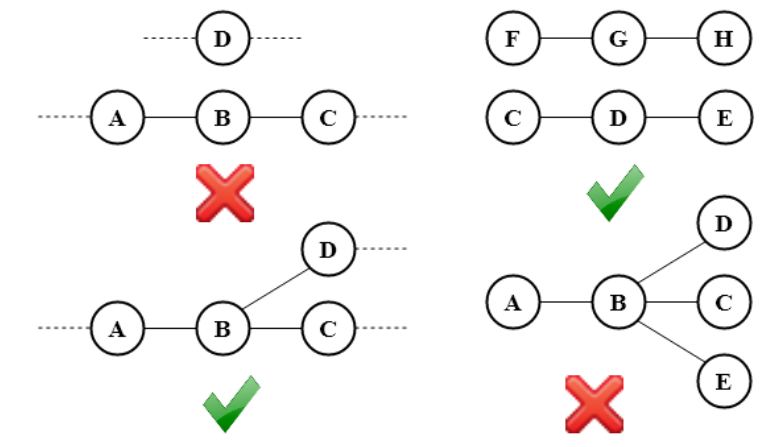
\includegraphics[width=0.8\textwidth]{Figuras/conexo.PNG}
        \centering\caption{Distintos tipos de redes de grafos.}
        \label{fig:conexidad}
    \end{figure}

    Para determinar si la red es conexa, se siguen los pasos del Algoritmo \ref{alg:connectedness}, y así se añaden nodos a una lista de zonas siempre que el nodo tenga un vecino en esa lista. Si un nodo posee un vecino en ambas listas, las listas se combinan, creando una nueva zona. Si la cantidad de zonas es uno entonces la red es fuertemente conexa. Una red ferroviaria disconexa puede resolverse mas rápido que una fuertemente conexa ya que no haría falta iterar entre todos los elementos para analizarlos sino solo los pertenecientes a dicho subgrafo.
        
    \begin{algorithm}[H]\captionsetup{labelfont={sc,bf}, labelsep=newline}
        \caption{Algoritmo de conexidad}
        \label{alg:connectedness}
        \begin{algorithmic}
            \STATE \{zones\} $\gets$ first node
            \FOR {node in \{nodes\}}
                \FOR {zone in \{zones\}}
                    \IF {node not in zones[zone]}
                        \IF {neighbours(node) in zones[zone]}
                            \STATE zones[zone] ADD node
                        \ELSE
                            \STATE Define new\_zone
                            \STATE zones[new\_zone] ADD node
                        \ENDIF
                    \ENDIF
                \ENDFOR
            \ENDFOR 
            \OUTPUT \{zones\}   
        \end{algorithmic}
    \end{algorithm}
        
    En las siguientes subsecciones se analizaran los elementos ferroviario descriptos en las clases \textit{FunctionalInfrastructure} y \textit{InfrastructureVisualizations}.